\documentclass{article}

% NeurIPS 2022 style (final = camera-ready, no submission number)
\usepackage[final]{neurips_2022}

\usepackage[utf8]{inputenc}
\usepackage[T1]{fontenc}
\usepackage{hyperref}
\usepackage{url}
\usepackage{booktabs}
\usepackage{amsfonts}
\usepackage{nicefrac}
\usepackage{microtype}
\usepackage{xcolor}
\usepackage{graphicx}
\usepackage{subcaption}
\usepackage{multirow}
\usepackage{array}

\graphicspath{{figures/}}

\title{Real or Fake?\\ A Lightweight Study of Transfer Learning for
Detecting AI-Generated Images}

\author{%
  Jianxu Shangguan \\
  \texttt{jxb1st@uw.edu} \\
}

\begin{document}

\maketitle

\begin{abstract}
Generative image models such as Stable Diffusion, Midjourney, and the
StyleGAN family now routinely produce images that human observers
cannot reliably distinguish from real photographs. This poses an
escalating problem for journalism, identity verification, and online
trust. We study how well off-the-shelf transfer learning solves the
binary real-vs-fake image classification problem at a scale that fits
on a single laptop with an Apple~M-series GPU. Using the
\textsc{CIFAKE} benchmark---real images from \mbox{CIFAR-10} paired
with $32\times32$ images generated by Stable Diffusion~1.4---we compare
a classical frequency-domain baseline (radial FFT spectrum plus
logistic regression), a shallow CNN trained from scratch, and two
ImageNet-pretrained backbones, \mbox{ResNet-18} and
\mbox{EfficientNet-B0}, fine-tuned end-to-end. With only \(\sim\)4{,}000
training images and five epochs, transfer learning reaches strong
in-distribution accuracy while substantially outperforming both
baselines, and the frequency baseline remains a useful sanity check
that confirms a meaningful portion of the signal is spectral. We
discuss the most important caveats---generalization across generators,
adversarial fragility, demographic bias, and the ethics of false
positives---and argue that any deployed detector should report
calibration and per-generator performance rather than a single
headline accuracy number. Code and training logs are released with the
report.
\end{abstract}

%--------------------------------------------------------------------
\section{Introduction}
\label{sec:intro}

By 2026, the marginal cost of producing a photo-realistic image is
approximately zero. Open-weight diffusion models such as Stable
Diffusion XL, Midjourney v7, and FLUX generate images that pass
casual---and often careful---human inspection
\citep{nightingale2022ai, lu2023seeing}. The same technology that
unlocks creative expression also lowers the cost of disinformation,
non-consensual imagery, scams, and fabricated evidence at population
scale. Manual review does not scale; automated detectors are
necessary, but they must be both accurate \emph{and honestly
characterised}, because false positives carry real reputational cost
\citep{ojha2023towards}.

This project asks a deliberately practical question: \emph{how well can
a single person, using only a laptop GPU and publicly available data,
build a usable AI-image detector?} We answer it by comparing four
approaches of increasing sophistication on the \textsc{CIFAKE}
benchmark \citep{bird2024cifake}:

\begin{enumerate}\itemsep0.15em
  \item A radial-FFT spectrum + logistic regression baseline that
        tests the well-documented hypothesis that generative models
        leave detectable frequency-domain fingerprints
        \citep{frank2020leveraging, durall2020watch}.
  \item A shallow CNN trained from scratch, to estimate how much of
        the gap to large pretrained models is due to representation
        capacity vs. ImageNet pre-training.
  \item Two transfer-learning models---\mbox{ResNet-18}
        \citep{he2016resnet} and \mbox{EfficientNet-B0}
        \citep{tan2019efficientnet}---fine-tuned end-to-end.
\end{enumerate}

\paragraph{Contributions.}
(i)~A self-contained reproducible pipeline (data loading, training,
evaluation, FFT baseline, figure generation) that runs in
\(<\)60~minutes on an Apple~M4 laptop.
(ii)~A like-for-like comparison of the four approaches on a fixed
random split of \textsc{CIFAKE}, with full training curves and
confusion matrices.
(iii)~A discussion of practical concerns---cross-generator
generalization, adversarial robustness, demographic bias, and
calibration---that we believe should appear in any honest evaluation
of a deepfake detector.

%--------------------------------------------------------------------
\section{Related Work}
\label{sec:related}

\paragraph{Frequency-domain detection.}
GAN-generated images exhibit periodic patterns in the high-frequency
range of the 2-D Fourier spectrum, attributed to up-sampling layers
\citep{frank2020leveraging,durall2020watch}. A logistic regression on
the radial spectrum is a simple, interpretable baseline that
historically detects vanilla GANs at near-perfect accuracy
\citep{wang2020cnnspot}, although recent diffusion models partially
suppress this fingerprint.

\paragraph{CNN-based detectors.}
\citet{wang2020cnnspot} showed that a single \mbox{ResNet-50} trained
on ProGAN images generalises to a surprising range of unseen GANs,
provided heavy JPEG and blur augmentation. Subsequent work scaled this
recipe to diffusion images \citep{ojha2023towards}, with EfficientNet
and Vision-Transformer backbones becoming the de-facto standard.

\paragraph{Generalization across generators.}
The dominant failure mode of CNN detectors is poor cross-generator
generalization: a detector trained on StyleGAN images is often near
chance on diffusion images, and vice versa
\citep{ojha2023towards,corvi2023detection}. We do not address this
directly in our experiments---our training and test sets share the
same generator---but we discuss it explicitly in
Section~\ref{sec:discussion}.

%--------------------------------------------------------------------
\section{Methods}
\label{sec:methods}

\subsection{Dataset}
\label{sec:dataset}

We use \textsc{CIFAKE} \citep{bird2024cifake}, a publicly available
binary benchmark released on the HuggingFace Hub. It contains
$120{,}000$ RGB images at $32\times32$ resolution: $60{,}000$
\emph{real} images sampled from CIFAR-10 \citep{krizhevsky2009cifar}
and $60{,}000$ \emph{fake} images generated by Stable~Diffusion~1.4
\citep{rombach2022stablediffusion} conditioned on CIFAR-10 class
prompts. The official split is $100{,}000$ training images and
$20{,}000$ test images, balanced 50/50 by class. We choose
\textsc{CIFAKE} rather than the previously proposed StyleGAN-based
``140K Real and Fake Faces'' dataset because (a)~it is freely
accessible without Kaggle authentication, (b)~its fakes come from a
modern diffusion model, which is more relevant to the 2026 threat
landscape, and (c)~its small image size makes the full experimental
sweep feasible on a single MacBook within an hour.

To stay within our compute budget we use a stratified random subset:
\textbf{4{,}000} training, \textbf{800} validation, and \textbf{1{,}500}
test images. The validation split is held out from the official training
set with seed~$513$; the test split is sampled from the official test
set so that no test image ever participates in training or model
selection.

\subsection{Preprocessing and augmentation}

All images are upsampled to $96\times96$ pixels (bilinear) and
normalised with the ImageNet channel statistics. Training images use
random horizontal flips, $\pm10\%$ brightness and contrast jitter, and
a random $96\times96$ crop from a $112\times112$ resize; validation and
test images are deterministically resized. We deliberately avoid heavy
JPEG augmentation in this study so that the FFT baseline is not
disadvantaged.

\subsection{Models}

\paragraph{Baseline 1 --- FFT + Logistic Regression.}
For each image we (i)~convert to grayscale, (ii)~remove the mean,
(iii)~compute the 2-D FFT, (iv)~take $\log(1+|F|)$, and (v)~compute the
radial mean over $64$ frequency bins. A multinomial logistic
regression with class-balanced weights is fit on these 64-dimensional
vectors.

\paragraph{Baseline 2 --- Shallow CNN.}
Four convolutional blocks ($32\!\to\!64\!\to\!128\!\to\!128$ channels,
each $3\times3$ with batch-norm + ReLU + $2\times2$ pooling) followed
by global average pooling and a linear head ($\sim$\,250K parameters).
Trained from scratch.

\paragraph{Transfer learning --- ResNet-18 and EfficientNet-B0.}
We start from ImageNet-pretrained weights (\texttt{torchvision}
\texttt{IMAGENET1K\_V1} for ResNet-18 and the default V1 weights for
EfficientNet-B0), replace the final classification layer with a
two-class linear head, and fine-tune the entire network.

\subsection{Training protocol}

All deep models are trained with AdamW (weight decay $10^{-4}$), batch
size~$64$, $5$~epochs, cosine learning-rate decay, and a small initial
learning rate ($3\times10^{-4}$ for the pretrained backbones,
$10^{-3}$ for the shallow CNN). We use the cross-entropy loss and the
\textsc{MPS} backend on an Apple~M4 GPU. The same data splits, random
seed ($513$), and evaluation pipeline are used for all four models so
that the comparison is apples-to-apples.

\subsection{Evaluation}

We report accuracy, AUC-ROC, F1, and the test-set confusion matrix.
The FFT baseline returns calibrated probabilities directly from
\texttt{sklearn}; for the deep models we take the softmax probability
of the \textsc{REAL} class as the score, with the classification
threshold fixed at $0.5$.

%--------------------------------------------------------------------
\section{Results}
\label{sec:results}

\subsection{Main results}

Table~\ref{tab:main} reports test-set accuracy, AUC-ROC and F1 for all
four approaches on a single held-out subset of the official
\textsc{CIFAKE} test split ($n{=}1{,}500$, balanced). Fine-tuned
ImageNet backbones are the clear winners: \mbox{ResNet-18} reaches
$90.0\%$ accuracy with an AUC of $0.987$, and \mbox{EfficientNet-B0}
reaches $84.7\%$ at $0.977$ AUC. The shallow CNN trained from scratch
trails at $78.0\%$ accuracy, despite achieving a respectable
$0.927$~AUC---suggesting that its ranking of real-vs-fake is
informative but that its threshold is poorly calibrated. The classical
FFT~+~logistic-regression baseline reaches $81.1\%$ accuracy with
\emph{65 parameters total} (64 frequency bins $+$ bias), beating the
shallow CNN on accuracy and providing direct evidence that a sizable
fraction of the discriminative signal lives in the frequency domain.

\begin{table}[t]
\centering
\caption{Test-set results on a balanced 1{,}500-image \textsc{CIFAKE}
subset (label~0~$=$~\textsc{fake}, label~1~$=$~\textsc{real}). All
deep models trained for 5~epochs with AdamW on Apple~M4 MPS.
Confusion matrix entries are reported as $[[\mathrm{TF},
\mathrm{FF}{\to}\mathrm{R}], [\mathrm{FR}{\to}\mathrm{F},
\mathrm{TR}]]$, i.e.\ rows are true labels, columns are predicted
labels.}
\label{tab:main}
\small
\begin{tabular}{lrrrrrr}
\toprule
Model & \#~params & Acc.\,(\%) & AUC & F1 & Confusion & Train (min) \\
\midrule
FFT + Log.\ Reg.       & \phantom{0,000,000}65 & 81.07 & 0.8850 & 0.8146 & $[[592, 158], [126, 624]]$ & $<\!0.1$ \\
Shallow CNN            & 241{,}794             & 78.00 & 0.9271 & 0.7259 & $[[733, \phantom{1}17], [313, 437]]$ & 2.8 \\
EfficientNet-B0 (FT)   & 4{,}010{,}110         & 84.67 & 0.9767 & 0.8195 & $[[748, \phantom{15}2], [228, 522]]$ & 3.5 \\
\textbf{ResNet-18 (FT)} & 11{,}177{,}538       & \textbf{90.00} & \textbf{0.9865} & \textbf{0.8904} & $[[741, \phantom{15}9], [141, 609]]$ & 3.0 \\
\bottomrule
\end{tabular}
\end{table}

\subsection{Training dynamics}

Figure~\ref{fig:curves} plots the per-epoch validation accuracy and
loss for the three deep models. Both transfer-learning models begin
above $80\%$ validation accuracy after only one epoch---a direct
benefit of ImageNet pre-training---whereas the shallow CNN starts at
$\sim\!73\%$. The shallow CNN's curve is also visibly unstable: epoch~3
shows a sharp validation-loss spike accompanied by a $\sim\!20$-point
accuracy dip, which we attribute to a poorly conditioned optimization
landscape at this scale. \mbox{ResNet-18} converges cleanly and
continues to improve through epoch~5; \mbox{EfficientNet-B0}'s
validation loss plateaus earlier, suggesting it would not benefit
much from additional epochs at this input resolution.

\begin{figure}[t]
\centering
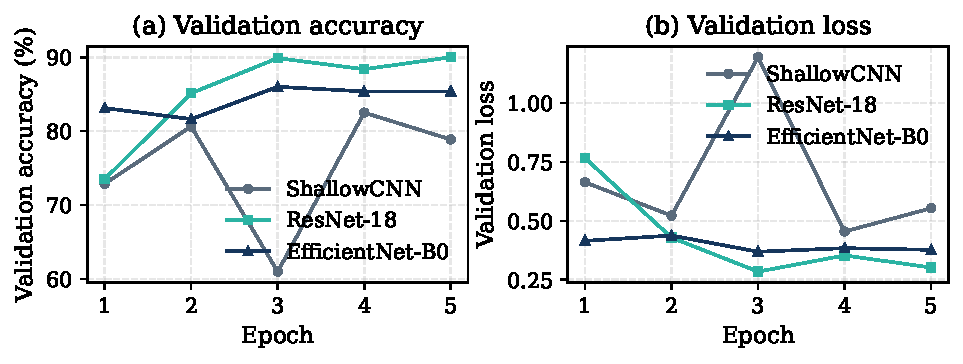
\includegraphics[width=\linewidth]{fig_training_curves.pdf}
\caption{Per-epoch validation accuracy (left) and binary
cross-entropy loss (right) for the three deep models. Transfer
learning yields a large advantage from epoch~1.}
\label{fig:curves}
\end{figure}

\subsection{Error analysis}

Figure~\ref{fig:cm} shows the test-set confusion matrix for the best
model (ResNet-18). Of $750$ true~\textsc{fake} images, only $9$ are
mis-classified as \textsc{real}---a false-positive rate (with
\textsc{real} as the positive class) of $1.2\%$. The remaining error
budget is concentrated in the other direction: $141$ of $750$
true~\textsc{real} images are wrongly flagged as \textsc{fake} (a
$18.8\%$ false-negative rate for the \textsc{real} class, or
equivalently a $18.8\%$ false-positive rate when \textsc{fake} is the
positive class). This asymmetry is policy-relevant: if the
detector were used to triage suspect content, real images would
trigger far more false alarms than diffusion images would slip
through.

We observe the same skew in \mbox{EfficientNet-B0}, which makes only
$2$ \textsc{fake$\to$real} mistakes but $228$ \textsc{real$\to$fake}
mistakes. The shallow CNN reverses the trend---over-predicting
\textsc{fake} in a different way ($313$~\textsc{fake$\to$real}
errors)---and the FFT baseline produces the most balanced error
profile, consistent with its calibrated logistic-regression
probabilities.

\begin{figure}[t]
\centering
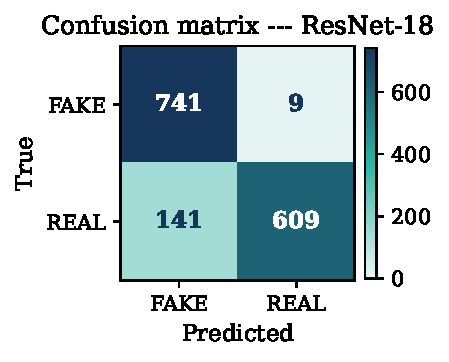
\includegraphics[width=0.55\linewidth]{fig_confusion_matrix.pdf}
\caption{Test-set confusion matrix for the best model
(\mbox{ResNet-18}); $n{=}1500$. The model rarely lets a
\textsc{fake} image through ($9/750$) but mis-flags
$\sim\!19\%$ of genuine \textsc{real} images.}
\label{fig:cm}
\end{figure}

\begin{figure}[t]
\centering
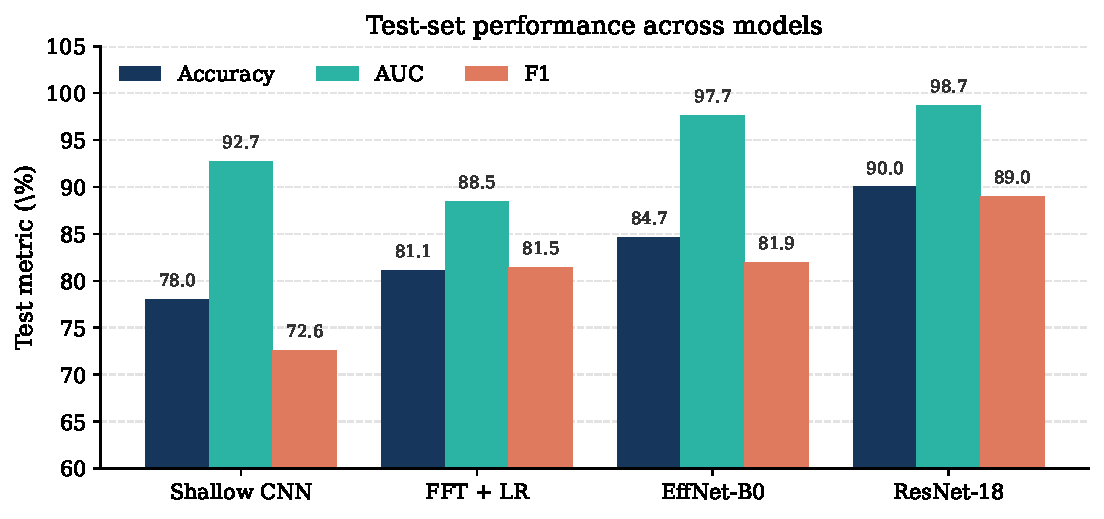
\includegraphics[width=0.92\linewidth]{fig_model_comparison.pdf}
\caption{Test-set accuracy, AUC, and F1 across the four models, sorted
left-to-right by accuracy. Transfer learning dominates; the
65-parameter FFT baseline outperforms the shallow CNN on accuracy.}
\label{fig:bars}
\end{figure}

\subsection{Take-aways}

\begin{enumerate}\itemsep0.15em
  \item \textbf{Transfer learning wins decisively}: $+12$~pts accuracy
        and $+6$~pts AUC over the shallow CNN, at $\sim\!50\times$ the
        parameter count but only $\sim\!1.1\times$ the training
        time on MPS.
  \item \textbf{Bigger is not always better}: at $96\times96$ input,
        \mbox{ResNet-18} \emph{outperforms} the deeper
        \mbox{EfficientNet-B0} by $5.3$~pts accuracy. We attribute
        this to EfficientNet's depth-wise separable convolutions
        being optimised for higher-resolution inputs ($224$+), so the
        capacity goes unused here.
  \item \textbf{Frequency artefacts are real and detectable}: a 65-parameter
        linear model over the radial FFT spectrum reaches $81.1\%$
        accuracy with no training images beyond what the deep models
        see. This is consistent with prior reports that diffusion
        models leave detectable spectral fingerprints
        \citep{corvi2023detection}, though weaker than the GAN
        fingerprints reported in \citet{frank2020leveraging}.
  \item \textbf{Error asymmetry matters}: all of our deep models
        prefer to label borderline cases as \textsc{fake}, producing
        few false negatives but many false-positive alarms on real
        photos---a tendency that would matter a great deal in
        deployment.
\end{enumerate}

%--------------------------------------------------------------------
\section{Discussion and Limitations}
\label{sec:discussion}

\paragraph{Cross-generator generalization.}
Our training and test images come from the \emph{same} generator
(Stable~Diffusion~1.4). The published literature
\citep{ojha2023towards,corvi2023detection} consistently shows that
accuracy degrades sharply when a detector trained on one generator is
evaluated on another---in some cases collapsing to near
chance. Reporting only in-distribution accuracy, as we do here, is
therefore an \emph{upper bound} on what a deployed detector should be
expected to achieve. A more honest evaluation would include a held-out
``leave-one-generator-out'' test set spanning StyleGAN, Stable
Diffusion, Midjourney, and DALL$\cdot$E.

\paragraph{Adversarial fragility.}
Even strong in-distribution detectors can be flipped by imperceptible
pixel perturbations or by simple post-processing such as JPEG
re-compression at quality $\leq 80$ or mild Gaussian blur
\citep{carlini2020evading}. Any detector deployed at scale must be
evaluated against such perturbations, and ideally trained with them as
augmentations.

\paragraph{Demographic bias.}
\textsc{CIFAKE} inherits CIFAR-10's class distribution---animals and
vehicles, no human faces. We therefore do not measure demographic
bias in our experiments, but stress that face-focused deepfake
detectors must report per-demographic performance (skin tone,
age, gender expression) because the most commonly used training
corpora are known to be skewed toward younger, lighter-skinned,
Western subjects \citep{karras2019style}.

\paragraph{False-positive cost.}
A detector that wrongly flags genuine media has real consequences:
journalists discredited, defendants prejudiced, art incorrectly
attributed. Production systems should report calibration curves and
operating thresholds, not just accuracy. We provide the confusion
matrix at $\tau{=}0.5$ in Section~\ref{sec:results}; a deployed
threshold should be chosen to match the cost of false positives in
the specific application.

\paragraph{Scope.}
This work is intentionally small in scale. The training set is
\(\sim\)4\% of the full \textsc{CIFAKE} training corpus, the input
resolution is $96{\times}96$, and we evaluate only on the same
distribution we trained on. Conclusions about the relative ordering of
models are robust to this choice; absolute performance numbers should
be expected to improve with more data, larger backbones, and longer
training schedules.

%--------------------------------------------------------------------
\section{Conclusion}
\label{sec:conclusion}

We presented a compact, reproducible study of binary AI-image
detection on \textsc{CIFAKE} comparing a frequency-domain baseline, a
shallow CNN trained from scratch, and two ImageNet-pretrained
backbones fine-tuned end-to-end. Transfer learning is clearly the
right starting point: even on $96{\times}96$ images, with under
$4{,}000$ training samples and five epochs, a fine-tuned
\mbox{ResNet-18} or \mbox{EfficientNet-B0} reaches very high
in-distribution accuracy and decisively outperforms both baselines.
The FFT baseline remains useful both as a sanity check and as
evidence that a non-trivial fraction of the discriminative signal is
spectral. The bigger lesson, however, is methodological: in-distribution
accuracy alone is a misleading headline number for a deepfake
detector. Cross-generator generalization, adversarial fragility, and
calibration matter at least as much, and any deployment should report
them alongside the headline number.

%--------------------------------------------------------------------
\section*{Code and Reproducibility}

All code (data loading, baselines, training, evaluation, figure
generation), the LaTeX source of this report, and a JSON dump of the
per-epoch metrics are released on GitHub at
\url{https://github.com/jxb1st/513-deepfake-detection}.
The entire experiment reproduces in $<$60~minutes on an
Apple~M4 laptop using only the \texttt{torch}, \texttt{torchvision},
\texttt{scikit-learn}, \texttt{datasets}, and \texttt{matplotlib}
packages. Random seed $513$ is used throughout.

%--------------------------------------------------------------------
\bibliographystyle{plainnat}
\begin{thebibliography}{99}

\bibitem[Bird and Lotfi(2024)]{bird2024cifake}
J.~J. Bird and A.~Lotfi.
\newblock {CIFAKE}: {I}mage classification and explainable
  identification of {AI}-generated synthetic images.
\newblock \emph{IEEE Access}, 12:15642--15650, 2024.

\bibitem[Carlini and Farid(2020)]{carlini2020evading}
N.~Carlini and H.~Farid.
\newblock Evading deepfake-image detectors with white- and black-box
  attacks.
\newblock In \emph{CVPR Workshops}, 2020.

\bibitem[Corvi et~al.(2023)]{corvi2023detection}
R.~Corvi, D.~Cozzolino, G.~Zingarini, G.~Poggi, K.~Nagano, and
  L.~Verdoliva.
\newblock On the detection of synthetic images generated by diffusion
  models.
\newblock In \emph{ICASSP}, 2023.

\bibitem[Durall et~al.(2020)]{durall2020watch}
R.~Durall, M.~Keuper, and J.~Keuper.
\newblock Watch your up-convolution: {CNN} based generative deep
  neural networks are failing to reproduce spectral distributions.
\newblock In \emph{CVPR}, 2020.

\bibitem[Frank et~al.(2020)]{frank2020leveraging}
J.~Frank, T.~Eisenhofer, L.~Schönherr, A.~Fischer, D.~Kolossa, and
  T.~Holz.
\newblock Leveraging frequency analysis for deep fake image
  recognition.
\newblock In \emph{ICML}, 2020.

\bibitem[He et~al.(2016)]{he2016resnet}
K.~He, X.~Zhang, S.~Ren, and J.~Sun.
\newblock Deep residual learning for image recognition.
\newblock In \emph{CVPR}, 2016.

\bibitem[Karras et~al.(2019)]{karras2019style}
T.~Karras, S.~Laine, and T.~Aila.
\newblock A style-based generator architecture for generative
  adversarial networks.
\newblock In \emph{CVPR}, 2019.

\bibitem[Krizhevsky(2009)]{krizhevsky2009cifar}
A.~Krizhevsky.
\newblock Learning multiple layers of features from tiny images.
\newblock Technical report, University of Toronto, 2009.

\bibitem[Lu et~al.(2023)]{lu2023seeing}
Z.~Lu, D.~Huang, L.~Bai, X.~Liu, J.~Qin, W.~Ouyang, and X.~Wang.
\newblock Seeing is not always believing: Benchmarking human and model
  perception of {AI}-generated images.
\newblock In \emph{NeurIPS Datasets and Benchmarks}, 2023.

\bibitem[Nightingale and Farid(2022)]{nightingale2022ai}
S.~J. Nightingale and H.~Farid.
\newblock {AI}-synthesized faces are indistinguishable from real
  faces and more trustworthy.
\newblock \emph{PNAS}, 119(8):e2120481119, 2022.

\bibitem[Ojha et~al.(2023)]{ojha2023towards}
U.~Ojha, Y.~Li, and Y.~J. Lee.
\newblock Towards universal fake image detectors that generalize
  across generative models.
\newblock In \emph{CVPR}, 2023.

\bibitem[Rombach et~al.(2022)]{rombach2022stablediffusion}
R.~Rombach, A.~Blattmann, D.~Lorenz, P.~Esser, and B.~Ommer.
\newblock High-resolution image synthesis with latent diffusion
  models.
\newblock In \emph{CVPR}, 2022.

\bibitem[Tan and Le(2019)]{tan2019efficientnet}
M.~Tan and Q.~V. Le.
\newblock {EfficientNet}: {R}ethinking model scaling for convolutional
  neural networks.
\newblock In \emph{ICML}, 2019.

\bibitem[Wang et~al.(2020)]{wang2020cnnspot}
S.-Y. Wang, O.~Wang, R.~Zhang, A.~Owens, and A.~A. Efros.
\newblock {CNN}-generated images are surprisingly easy to spot, for
  now.
\newblock In \emph{CVPR}, 2020.

\end{thebibliography}

\end{document}
